\pdfbookmark{Общая характеристика работы}{characteristic}             % Закладка pdf
\section*{Общая характеристика работы}

\newcommand{\actuality}{\pdfbookmark[1]{Актуальность темы исследования}{actuality}\underline{\textbf{\actualityTXT}}}
\newcommand{\progress}{\pdfbookmark[1]{Степень разработанности темы исследования}{progress}\underline{\textbf{\progressTXT}}}
\newcommand{\aim}{\pdfbookmark[1]{Цели}{aim}\underline{{\textbf\aimTXT}}}
\newcommand{\tasks}{\pdfbookmark[1]{Задачи}{tasks}\underline{\textbf{\tasksTXT}}}
\newcommand{\aimtasks}{\pdfbookmark[1]{Цели и задачи}{aimtasks}\aimtasksTXT}
\newcommand{\novelty}{\pdfbookmark[1]{Научная новизна}{novelty}\underline{\textbf{\noveltyTXT}}}
\newcommand{\influence}{\pdfbookmark[1]{Теоретическая и практическая значимость работы}{influence}\underline{\textbf{\influenceTXT}}}
\newcommand{\methods}{\pdfbookmark[1]{Методология и методы исследования}{methods}\underline{\textbf{\methodsTXT}}}
\newcommand{\defpositions}{\pdfbookmark[1]{Положения, выносимые на защиту}{defpositions}\underline{\textbf{\defpositionsTXT}}}
\newcommand{\reliability}{\pdfbookmark[1]{Достоверность}{reliability}\underline{\textbf{\reliabilityTXT}}}
\newcommand{\contribution}{\pdfbookmark[1]{Личный вклад}{contribution}\underline{\textbf{\contributionTXT}}}
\newcommand{\publications}{\pdfbookmark[1]{Публикации}{publications}\underline{\textbf{\publicationsTXT}}}


{\actuality} 
В современном мире происходит значительный рост данных, которые требуют анализа. Графы используются в качестве структуры данных для представления больших объемов информации в компактной и удобной для анализа форме во многих областях, например, в биоинформатике, в графовых базах данных, при статическом анализе программ. При этом оказывается необходимым выявлять сложные зависимости между вершинами графа, которые выражаются путями между ними. Поэтому очень важен широкий класс задач, посвященный поиску путей в графах. Чтобы описать свойства искомых путей в графе, необходимо задать определенные ограничения на них. Данные ограничения формулируются в виде запроса к графу, а ответом на запрос является информация о существовании путей, удовлетворяющих данным ограничениям между каждой парой вершин. Кроме того, в некоторых областях, в качестве доказательства существования таких путей необходимо предъявить все или хотя бы один из них.

Для описания ограничений на пути в помеченном графе естественно выделять пути с помощью формальных грамматик (регулярные выражения, контекстно-свободные грамматики) над алфавитом, содержащим метки на ребрах этого графа. В настоящее время активно исследуются ограничения в виде контекстно-свободных (КС) грамматик, так как они позволяют описывать более широкий класс запросов (КС-запросов), чем регулярные выражения. Однако большинство существующих алгоритмов вычисления КС-запросов имеют низкую производительность на больших графах, что затрудняет их применение на практике.

Одним из распространённых способов улучшения производительности алгоритмов на графах является их формулирование в терминах операций линейной алгебры над матрицами и векторами. Для тех алгоритмов, которые позволяют найти такую формулировку, имеется возможность применить широкий класс оптимизаций, например, разреженное представление матриц и параллельное вычисление. Кроме того, данные алгоритмы зачастую просты в реализации, так как позволяют использовать существующие реализации для вычисления операций над матрицами. Таким образом, формулирование различных алгоритмов на графах в терминах операций линейной алгебры над матрицами и векторами является перспективным направлением.

Однако возможность использования операций линейной алгебры в задачах поиска путей с КС-ограничениями в графах в настоящее время не исследована. Таким образом, для КС-ограничений актуальна разработка и исследование свойств алгоритмов поиска путей, использующих различные операции линейной алгебры.

%Кроме того, в данной области КС-грамматика приводится в нормальную форму, что способствует её разрастанию и увеличивает время анализа. Таким образом, перспективным направлением является исследование возможности использования такой матричной операции, как произведение Кронекера. Использование данной операции позволит работать с КС-грамматиками произвольного вида без необходимости их преобразования. Таким образом, алгоритм поиска путей с КС-ограничениями в графах, использующий произведение Кронекера может позволить получить еще больший прирост производительности за счёт отсутсвия разрастания размеров грамматики.


%Обзор, введение в тему, обозначение места данной работы в
%мировых исследованиях и~т.\:п., можно использовать ссылки на~другие
%работы~\autocite{Gosele1999161}
%(если их~нет, то~в~автореферате
%автоматически пропадёт раздел <<Список литературы>>). Внимание! Ссылки
%на~другие работы в~разделе общей характеристики работы можно
%использовать только при использовании \verb!biblatex! (из-за технических
%ограничений \verb!bibtex8!. Это связано с тем, что одна
%и~та~же~характеристика используются и~в~тексте диссертации, и в
%автореферате. В~последнем, согласно ГОСТ, должен присутствовать список
%работ автора по~теме диссертации, а~\verb!bibtex8! не~умеет выводить в~одном
%файле два списка литературы).
%При использовании \verb!biblatex! возможно использование исключительно
%в~автореферате подстрочных ссылок
%для других работ командой \verb!\autocite!, а~также цитирование
%собственных работ командой \verb!\cite!. Для этого в~файле
%\verb!common/setup.tex! необходимо присвоить положительное значение
%счётчику \verb!\setcounter{usefootcite}{1}!.


{\progress}
Множество работ посвящены формулированию классических алгоритмов на графах в терминах операций линейной алгебры. Например, такая формулировка была найдена для таких алгоритмов, как поиск в ширину, алгоритм Дейкстры, алгоритм Беллмана-Форда, поиск наибольшего паросочетания в двудольном графе и т.д. Кроме того, существует стандарт GraphBLAS, который определяет базовые строительные блоки для графовых алгоритмов на языке линейной алгебры. GraphBLAS основан на том, что разреженная матрица может использоваться для представления графов в виде матрицы смежности или матрицы инцидентности. Однако формулировка в терминах операций линейной алгебры для алгоритмов вычисления КС-запросов на графах в настоящее время не найдена.

Существует классическое исследование Лесли Вэлианта, посвященное синтаксическому анализу КС-грамматик с использованием матричных операций. Однако изложенный в нём алгоритм позволяет производить анализ только над строками, что эквивалентно анализу частного случая графов --- линейных помеченных графов. Кроме того, существуют исследования Филиппа Брэдфорда посвященные поиску кратчайших путей в графе с КС-ограничениями. Алгоритмы, представленные в данных исследованиях предназначены для частного случая КС-грамматик и/или частного случая графов. Таким образом, данные алгоритмы не применимы к поиску путей с произвольными КС-ограничениями в произвольных графах.

Задаче поиска путей с КС-ограничениями в произвольных графах посвящены работы Семёна Григорьева, Джелле Хеллингса, Сяованга Чжана, Сиро Медейроса. В данных исследованиях используются подходы, основанные на различных алгоритмах синтаксического анализа (LR, LL, GLL, CYK). Однако, данные алгоритмы сформулированы не в терминах операций линейной алгебры над матричами и векторами. Впервые вопросом о возможности нахождения матричного алгоритма вычисления КС-запросов к графам задался Яннакакис в своем исследовании о применимости методов из теории графов в теории баз данных. Он указывал на то, что алгоритм Вэлианта может быть расширен для работы с графами без циклов, однако сомневался в возможности расширения до произвольных графов.

Таким образом, на текущий момент не существует алгоритма вычисления произвольных КС-запросов к произвольным графам, выраженного через операции линейной алгебры. Поэтому необходимо дальнейшее исследование возможности разработки таких алгоритмов.
%Этот раздел должен быть отдельным структурным элементом по
% ГОСТ, но он, как правило, включается в описание актуальности
% темы. Нужен он отдельным структурынм элемементом или нет ---
% смотрите другие диссертации вашего совета, скорее всего не нужен.

{\aim} данной работы является разработка алгоритмов вычисления КС-запросов к графам, использующих операции линейной алгебры.

Достижение поставленной цели обеспечивается решением следующих {\tasks}:
\begin{enumerate}[beginpenalty=10000] % https://tex.stackexchange.com/a/476052/104425
  \item Разработать подход к вычислению КС-запросов к графам, использующий операции линейной алгебры.
  \item Разработать семейство алгоритмов вычисления КС-запросов к графам, использующих предложенный подход и позволяющих предоставлять искомые пути.
  \item Разработать семейство алгоритмов вычисления КС-запросов к графам, использующий предложенный подход и не требующего преобразований входной КС-грамматики.
  \item Провести экспериментальное исследование разработанных алгоритмов.
\end{enumerate}


{\novelty}
\begin{enumerate}[beginpenalty=10000] % https://tex.stackexchange.com/a/476052/104425
	
	\item Подход, предложенный в диссертации, отличается от подходов, использованных в работах Семёна Григорьева, Сяованга Чжана, Джелле Хеллингса, Филиппа Брэдфорда и Сиро Медейроса активным использованием матричных операций в процессе вычисления запросов. Это позволяет применять широкий класс оптимизаций для вычисления матричных операций и дает возможность автоматически распараллеливать вычисления за счёт существующих решений.
	
	\item Задача вычисления КС-запросов к графам впервые сведена к вычислению операций линейной алгебры и получены соответсвующие алгоритмы.
	
	\item Алгоритмы, предложенный в диссертации, отличается от алгоритмов, предложенных в работах Семёна Григорьева, Сяованга Чжана, Джелле Хеллингса, Филиппа Брэдфорда и Сиро Медейроса возможностью работать с произвольными КС-грамматиками без необходимости приводить их в нормальную форму. Таким образом, удаётся избежать значительного увеличения размеров входной грамматики, от которой напрямую зависит временная сложность данных алгоритмов.
	
	\item Экспериментальное исследование алгоритмов вычисления КС-запросов к графам, использующих операции линейной алгебры проводится впервые и позволяет судить о применимости на практике разработанных алгоритмов.
	
\end{enumerate}

{\influence} 
Теоретическая значимость диссертационного исследования заключается в разработке подхода к вычислению КС-запросов к графам, использующего операции линейной алгебры, в разработке формальных алгоритмов, использующих данный подход, а также в формальном доказательстве завершаемости и корректности разработанных алгоритмов.

Полученные в ходе исследования реализации могут быть использованы для интеграции с такими графовыми базами данных, как RedisGraph. Это добавит возможность вычислять КС-запросы к этим базам данных.

{\methods} Методология исследования основана на подходе использования операций линейной алгебре при анализе графов, который начал активно развиваться с 2013 года в связи с созданием стандарта GraphBLAS. Данный стандарт определяет базовые строительные блоки для графовых алгоритмов на языке линейной алгебры. GraphBLAS основан на том, что разреженная матрица может использоваться для представления графов в виде матрицы смежности или матрицы инцидентности. На текущий момент множество классических алгоритмов из теории графов были сформулированы в терминах линейной алгебры.

Однако для большинства задач анализа графов такая формулировка ещё не найдена. Одной из таких задач является поиск путей в графе с ограничениями в виде КС-грамматик. Данная задача использует подход к анализу строк с помощью теории формальных языков и грамматик, который начал активно развиваться в 50-х годах 20-го века в связи с изучением естественных языков (работы Н.~Хомского). В последствии этот подход получил широкое распространение в различных областях, в том числе и связанных с анализом графов.
При этом основными элементами данного подхода являются алфавит и грамматика исследуемого языка, выступающего в качестве ограничения на искомые пути в графе. Решаемые в связи с этим задачи связаны с поиском эффективных алгоритмов нахождения путей, удовлетворяющих заданным ограничениям.

Доказательство завершаемости и корректности предложенного алгоритма проводится с применением линейной алгебры, теории формальных языков, теории графов и теории сложности алгоритмов.

{\defpositions}
\begin{enumerate}[beginpenalty=10000] % https://tex.stackexchange.com/a/476052/104425
	\item Разработан подход к вычислению КС-запросов к графам, использующий операции линейной алгебры.
	\item Разработано семейство алгоритмов вычисления КС-запросов к графам, использующих предложенный подход и позволяющих предоставлять искомые пути. Доказана завершаемость и корректность предложенных алгоритмов.
	\item Разработано семейство алгоритмов вычисления КС-запросов к графам, использующий предложенный подход и не требующего преобразований входной КС-грамматики. Доказана завершаемость и корректность предложенных алгоритмов.
	\item Проведено экспериментальное исследование разработанных алгоритмов.
\end{enumerate}

{\reliability} 
Достоверность и обоснованность результатов исследования опирается на использование формальных методов исследуемой области, выполнение формальных доказательств и инженерные эксперименты.

Основные результаты работы были доложены на ряде международных научных конференций: GRADES'18, GRADES'20, ADBIS’20, SIGMOD'21(еще не приняли). А также разработка предложенных алгоритмов была поддержана грантом РНФ \textnumero 18-11-00100 и грантом РФФИ \textnumero 19-37-90101.

%{\contribution} Автор принимал активное участие \ldots

{\publications} Все результаты диссертации изложены в 7~\cite{1,2,3,4,5,6,7} научных работах, которые содержат основные результаты работы. Из них 2 работы~\cite{6,7} индексируются ВАК и 6 работ~\cite{1,2,3,4,5,6} индексируются Scopus. Работы~\cite{1,2,3,4,6,7} написаны в соавторстве. В~\cite{1,6,7} Р.~Азимову принадлежит разработка алгоритма, доказательство его корректности и завершаемости, реализация алгоритма, работа над текстом. В~\cite{2} Р.~Азимову принадлежит разработка алгоритма, доказательство его корректности и завершаемости, работа над текстом. В~\cite{3,4} Р.~Азимову принадлежит работа над доказательствами корректности и завершаемости алгоритма, работа над текстом.

\newcounter{firstbib}

\begin{thebibliography}{99}
	\bibitem{1} Azimov R. Context-Free Path Querying by
	Matrix Multiplication / Azimov R., Grigorev S. // In Proceedings of the
	1st Joint International Workshop on Graph Data Management Experiences \&
	Systems (GRADES) and Network Data Analytics (NDA) (GRADES-NDA’18)
	\bibitem{2} Azimov R. Context-Free Path Querying with Single-Path Semantics by
	Matrix Multiplication / Terekhov A., Khoroshev A., Azimov R., Grigorev S. // In Proceedings of the
	3rd Joint International Workshop on Graph Data Management Experiences \&
	Systems (GRADES) and Network Data Analytics (NDA) (GRADES-NDA’20)
	\bibitem{3} Azimov R. Context-Free Path Querying by Kronecker
	Product / Orachev E., Epelbaum I., Azimov R., Grigorev S. // In Proceedings of the
	24th European Conference on Advances in Databases and Information Systems (ADBIS’20)
	\bibitem{4} Azimov R. Context-Free Path Querying by Kronecker
	Product большая версия / Orachev E., Epelbaum I., Azimov R., Grigorev S. // In Proceedings of the (SIGMOD’21)
	
	\bibitem{5} Azimov R. Ненаписанная работа матричный алгоритм по всем путям
	
	\bibitem{6} Azimov R. Path Querying with Conjunctive Grammars by Matrix Multiplication / Azimov R., Grigorev S. //Programming and Computer Software. – 2019. – Vol. 45. – №. 7. – pp. 357-364.
	\setcounter{firstbib}{\value{enumiv}}
	
	\bibitem{7} Азимов Р. Ш. Синтаксический анализ графов с использованием конъюнктивных грамматик / Азимов Р., Григорьев С. // Труды ИСП РАН, 2018, том 1 вып. 2, с. 3-4.
	
\end{thebibliography} % Характеристика работы по структуре во введении и в автореферате не отличается (ГОСТ Р 7.0.11, пункты 5.3.1 и 9.2.1), потому её загружаем из одного и того же внешнего файла, предварительно задав форму выделения некоторым параметрам

%Диссертационная работа была выполнена при поддержке грантов \dots

%\underline{\textbf{Объем и структура работы.}} Диссертация состоит из~введения,
%четырех глав, заключения и~приложения. Полный объем диссертации
%\textbf{ХХХ}~страниц текста с~\textbf{ХХ}~рисунками и~5~таблицами. Список
%литературы содержит \textbf{ХХX}~наименование.

\pdfbookmark{Содержание работы}{description}                          % Закладка pdf
\section*{Содержание работы}
Во \underline{\textbf{введении}} обосновывается актуальность
исследований, проводимых в~рамках данной диссертационной работы,
приводится обзор научной литературы по~изучаемой проблеме,
формулируется цель, ставятся задачи работы, излагается научная новизна
и практическая значимость представляемой работы. В~последующих главах
сначала описывается общий принцип, позволяющий \dots, а~потом идёт
апробация на частных примерах: \dots  и~\dots.


\underline{\textbf{Первая глава}} посвящена \dots

 картинку можно добавить так:
\begin{figure}[ht]
    \centerfloat{
        \hfill
        \subcaptionbox{\LaTeX}{%
            
\includegraphics[scale=0.27]{latex}}
        \hfill
        \subcaptionbox{Knuth}{%
            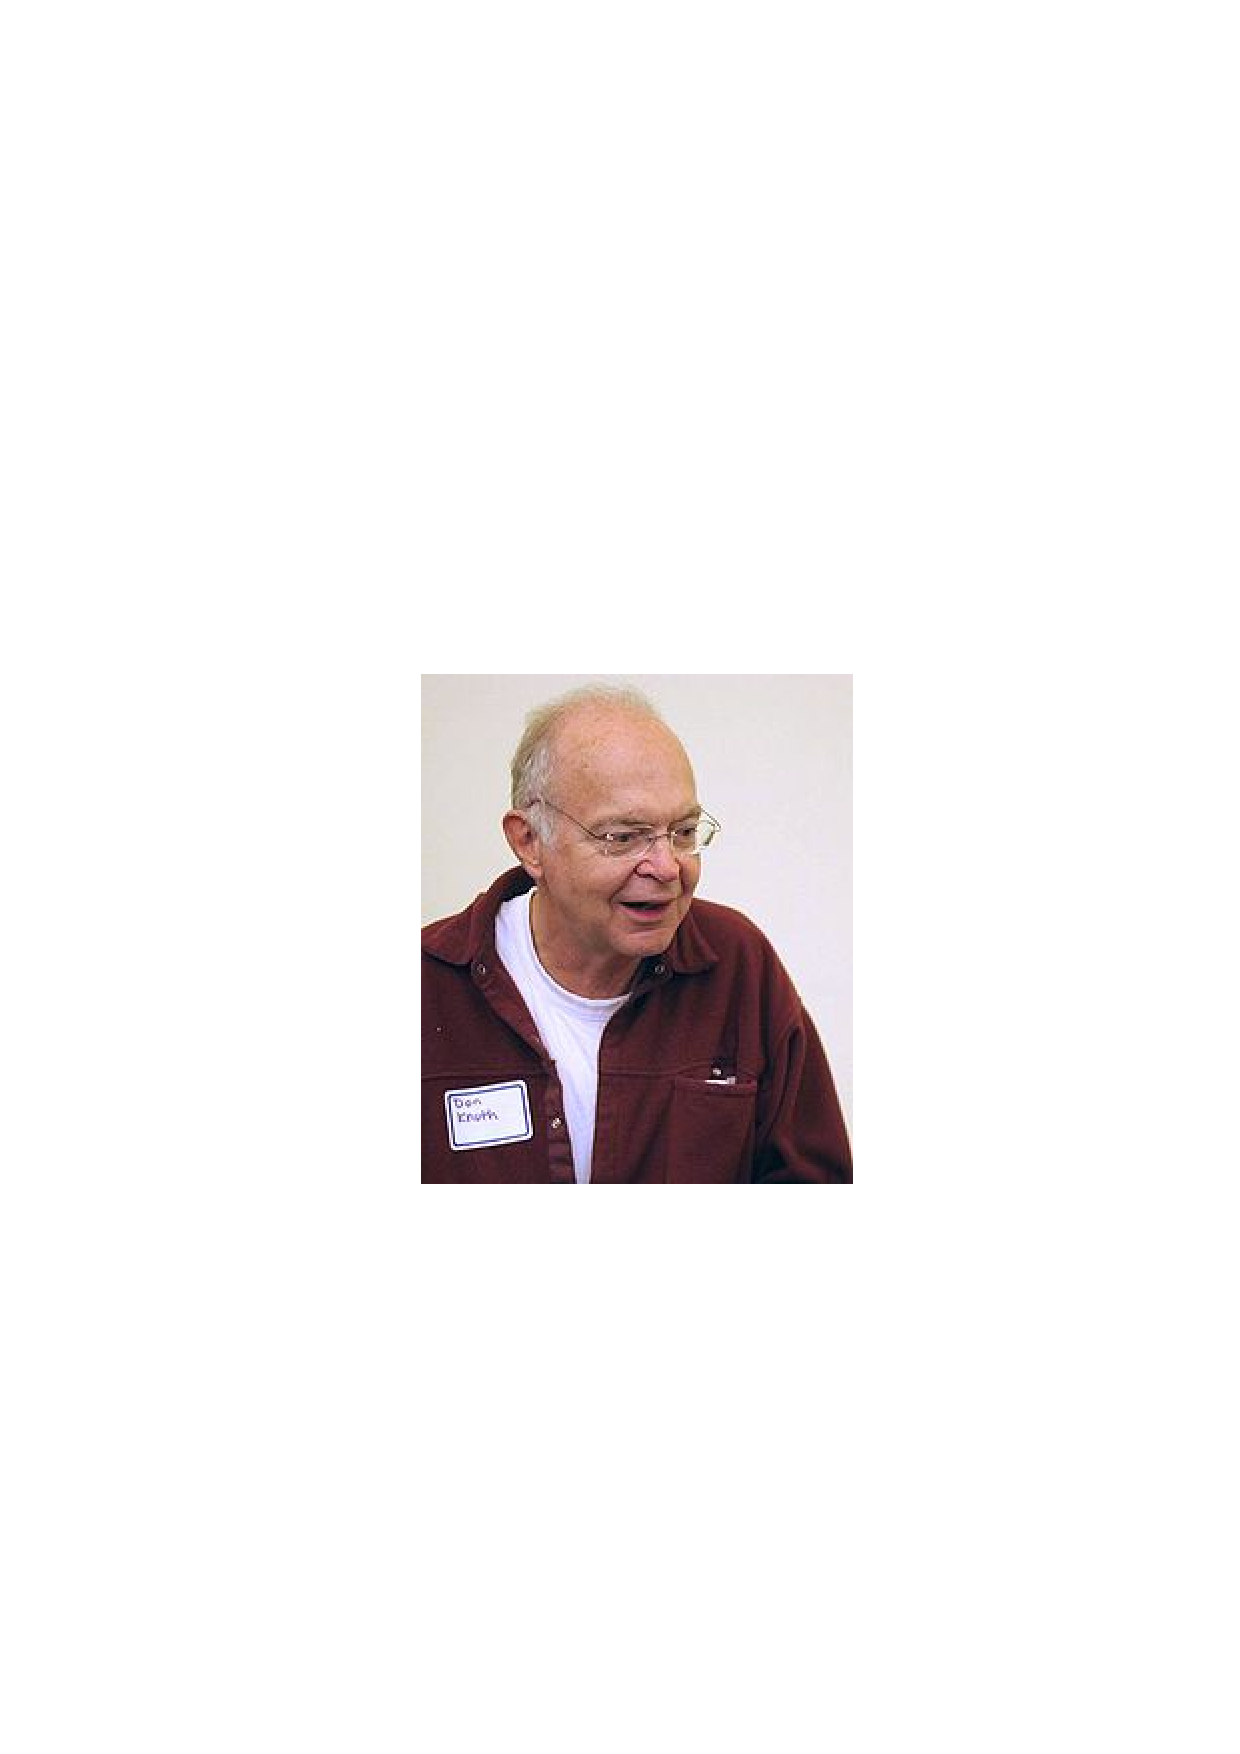
\includegraphics[width=0.25\linewidth]{knuth1}}
        \hfill
    }
    \caption{Подпись к картинке.}\label{fig:latex}
\end{figure}

Формулы в строку без номера добавляются так:
\[
  \lambda_{T_s} = K_x\frac{d{x}}{d{T_s}}, \qquad
  \lambda_{q_s} = K_x\frac{d{x}}{d{q_s}},
\]

\underline{\textbf{Вторая глава}} посвящена исследованию

\underline{\textbf{Третья глава}} посвящена исследованию

Можно сослаться на свои работы в автореферате. Для этого в файле
\verb!Synopsis/setup.tex! необходимо присвоить положительное значение
счётчику \verb!\setcounter{usefootcite}{1}!. В таком случае ссылки на
работы других авторов будут подстрочными.
Изложенные в третьей главе результаты опубликованы в~\cite{vakbib1, vakbib2}.
Использование подстрочных ссылок внутри таблиц может вызывать проблемы.

В \underline{\textbf{четвертой главе}} приведено описание

\FloatBarrier
\pdfbookmark{Заключение}{conclusion}                                  % Закладка pdf
В \underline{\textbf{заключении}} приведены основные результаты работы, которые заключаются в следующем:
%% Согласно ГОСТ Р 7.0.11-2011:
%% 5.3.3 В заключении диссертации излагают итоги выполненного исследования, рекомендации, перспективы дальнейшей разработки темы.
%% 9.2.3 В заключении автореферата диссертации излагают итоги данного исследования, рекомендации и перспективы дальнейшей разработки темы.
\begin{enumerate}
  \item Разработан подход к вычислению КС-запросов к графам, использующий операции линейной алгебры.
  \item Разработано семейство алгоритмов вычисления КС-запросов к графам, использующих предложенный подход и позволяющих предоставлять искомые пути. Доказана завершаемость и корректность предложенных алгоритмов.
  \item Разработано семейство алгоритмов вычисления КС-запросов к графам, использующий предложенный подход и не требующего преобразований входной КС-грамматики. Доказана завершаемость и корректность предложенных алгоритмов.
  \item Проведено экспериментальное исследование разработанных алгоритмов.
\end{enumerate}


\pdfbookmark{Литература}{bibliography}                                % Закладка pdf
При использовании пакета \verb!biblatex! список публикаций автора по теме
диссертации формируется в разделе <<\publications>>\ файла
\verb!common/characteristic.tex!  при помощи команды \verb!\nocite!

\ifdefmacro{\microtypesetup}{\microtypesetup{protrusion=false}}{} % не рекомендуется применять пакет микротипографики к автоматически генерируемому списку литературы
\urlstyle{rm}                               % ссылки URL обычным шрифтом
\ifnumequal{\value{bibliosel}}{0}{% Встроенная реализация с загрузкой файла через движок bibtex8
  \renewcommand{\bibname}{\large \bibtitleauthor}
  \nocite{*}
  \insertbiblioauthor           % Подключаем Bib-базы
  %\insertbiblioexternal   % !!! bibtex не умеет работать с несколькими библиографиями !!!
}{% Реализация пакетом biblatex через движок biber
  % Цитирования.
  %  * Порядок перечисления определяет порядок в библиографии (только внутри подраздела, если `\insertbiblioauthorgrouped`).
  %  * Если не соблюдать порядок "как для \printbibliography", нумерация в `\insertbiblioauthor` будет кривой.
  %  * Если цитировать каждый источник отдельной командой --- найти некоторые ошибки будет проще.
  %
  %% authorvak
  \nocite{vakbib1}%
  \nocite{vakbib2}%
  %
  %% authorwos
  \nocite{wosbib1}%
  %
  %% authorscopus
  \nocite{scbib1}%
  %
  %% authorconf
  \nocite{confbib1}%
  \nocite{confbib2}%
  %
  %% authorother
  \nocite{bib1}%
  \nocite{bib2}%

  \ifnumgreater{\value{usefootcite}}{0}{
    \begin{refcontext}[labelprefix={}]
      \ifnum \value{bibgrouped}>0
        \insertbiblioauthorgrouped    % Вывод всех работ автора, сгруппированных по источникам
      \else
        \insertbiblioauthor      % Вывод всех работ автора
      \fi
    \end{refcontext}
  }{
  \ifnum \value{citeexternal}>0
    \begin{refcontext}[labelprefix=A]
      \ifnum \value{bibgrouped}>0
        \insertbiblioauthorgrouped    % Вывод всех работ автора, сгруппированных по источникам
      \else
        \insertbiblioauthor      % Вывод всех работ автора
      \fi
    \end{refcontext}
  \else
    \ifnum \value{bibgrouped}>0
      \insertbiblioauthorgrouped    % Вывод всех работ автора, сгруппированных по источникам
    \else
      \insertbiblioauthor      % Вывод всех работ автора
    \fi
  \fi
  %  \insertbiblioauthorimportant  % Вывод наиболее значимых работ автора (определяется в файле characteristic во второй section)
  \begin{refcontext}[labelprefix={}]    \insertbiblioexternal            % Вывод списка литературы, на которую ссылались в тексте автореферата
  \end{refcontext}
  }
}
\ifdefmacro{\microtypesetup}{\microtypesetup{protrusion=true}}{}
\urlstyle{tt}                               % возвращаем установки шрифта ссылок URL
